Ahora se necesita modificar un elemento del arreglo \texttt{A} original y seguir contestando consultas en rangos. Se obtiene un nuevo arreglo \texttt{A'} que difiere del original solo en una posici\'on.

Deseamos obtener un segment tree para el arreglo \texttt{A'}, pero sin construirlo desde cero, en vez de eso, vamos a utilizar el segment tree ya existente. Debemos modificar nuestra estructura de tal manera que los resultados que precalculamos para cada nodo sean los correspondientes al nuevo arreglo \texttt{A'}. A esta operaci\'on se le conoce como actualizaci\'on de posici\'on.\\

\noindent\textit{?`Cu\'ales son los nodos cuyo valor hay que modificar?} \\
Primeramente si $p$ es la posici\'on que vamos a modificar, entonces debemos actualizar el valor del nodo hoja cuyo intervalo es $[p, p]$, porque su valor depende totalmente del n\'umero en la posici\'on $p$ del arreglo. Pero cuando construimos el segment tree original, el valor del padre de ese nodo fue calculado como la suma de los valores de dicho nodo y el otro hijo, por lo que si modificamos el valor del nodo, hay que modificar el valor del padre.

Pero lo mismo pasa con el padre del padre, y con el siguente nodo en direcci\'on a la ra\'iz... En conclusi\'on, se modifica el v\'ertice $v$, cuyo rango es $[p, p]$, y todos los dem\'as nodos en el camino entre $v$ y la ra\'iz del \'arbol.

Por ejemplo, si vamos a modificar la posici\'on $p = 3$ y le vamos a colocar el valor $5$, modificamos el nodo de rango $[3, 3]$ que antes ten\'ia el valor $1$, ahora le colocamos el valor $5$. Luego actualizamos el valor del nodo de rango $[1, 3]$. Ahora ser\'a $5 + 5 = 10$. Por \'ultimo actualizamos el valor de la ra\'iz: $10 + 9 = 19$.

\begin{minipage}{\columnwidth}
    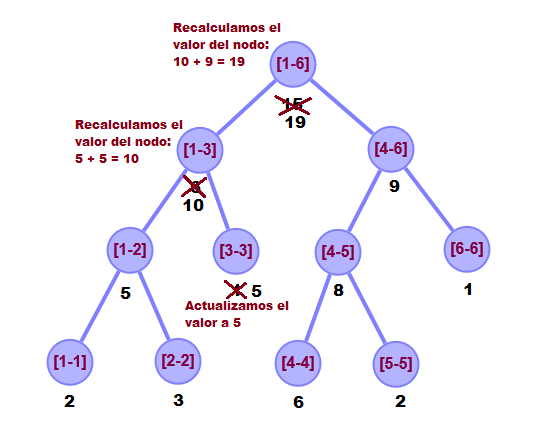
\includegraphics[width=\linewidth]{imag/segment_tree_update}
    \label{fig:example_st_casos}
\end{minipage}

Observe que el segment tree resultante es igual al segment tree que hubi\'esemos construido si el arreglo original fuera $\{2, 3, \underline{5}, 6, 2, 1\}$.

En el caso de la actualizaci\'on de posici\'on \textbf{los valores que se calculan para cada nodo en las actualizaciones s\'i modifican los valores de los nodos del segment tree}.

Ahora hay que formalizar el m\'etodo de la actualizaci\'on de posici\'on para posteriormente implementarlo. 

\begin{corollary}[Actualizaci\'on de Posici\'on]
    Nos dan una posici\'on $p$ a modificar, y un valor $x$ que es el nuevo valor. El procedimiento es recursivo y comienza en el nodo ra\'iz. Cuando llegamos a un v\'ertice $v$ cuyo rango es $[l, r]$ tenemos tres casos posibles:

    \begin{enumerate}
        \item{
            \textit{Si el intervalo $[l, r]$ del nodo est\'a completamente DENTRO del intervalo $[p, p]$ (Esto solo se cumple si $l = r = p$):}  Como $l = r = p$ entonces el nodo actual es el nodo hoja cuyo intervalo es $[p, p]$. El nuevo valor del nodo ser\'a $x$, el cual se retorna.
        }
        \item{
            \textit{Si el intervalo $[l, r]$ del nodo est\'a completamente FUERA del intervalo $[p, p]$:} No se modifica el nodo y se retorna el valor que ya ten\'ia.
        }
        \item{
            \textit{Si no se cumple NINGUNA de las condiciones anteriores:} Entonces llevamos a cabo este procedimiento en los hijos del nodo actual y luego combinamos la respuesta de cada v\'ertice hijo, para recalcular el valor del nodo actual con los valores retornados.
        }
    \end{enumerate}
\end{corollary}

\noindent\textit{?`Cuál es la complejidad temporal de una actualizaci\'on de posici\'on?} \\
Al igual que en los m\'etodos anteriores, la complejidad temporal depende de la cantidad de v\'ertices del \'arbol que ser\'an visitados. Como solo se modifican los nodos en el camino desde el vertice $v$ hasta la ra\'iz utilizando ambos hijos para recalcular los valores, en cada nivel del \'arbol se visitan a lo m\'as dos nodos. La cantidad de nodos total ser\'a como m\'aximo $2 \cdot \log_2(n) + 2 = O(\log n)$.


